\chapter{Wstęp}
\markboth{Wstęp}{Wstęp}
\label{wstep}

Od zarania dziejów ludzkość interesowała się , który rozpalał umysły myślicieli oraz inspirował wynalazców. Już w starożytności opisano wynalazek znany dziś pod nazwą gimbal, a pitagorejczycy rozpatrywali ruch obrotowy Ziemi. Na przestrzeni kolejnych wieków wciąż pozostawał on w umysłach znakomitych uczonych, takich jak Isaac Newton (1642--1727) \cite{newton}, Mikołaj Kopernik (1473--1543) \cite{copernicus1965revolutionibus} czy Girolamo Cardano (1501--1573) \cite{cardano}, który częściowo stworzył, a także opisał specjalny typ zawieszenia nazwanego później jego nazwiskiem -- kluczową część ówczesnych kompasów oraz żyroskopów i przyczynek do zaprojektowania przegubu Cardana, nieodzownego elementu wielu współczesnych mechanizmów napędowych \cite{przegCard}.

{\red
  Wstęp stanowi wprowadzenie w~podejmowane zagadnienia, powinien więc ,,umiejscawiać tematykę pracy''. Stąd należy sięgnąć do tego, co zostało dotychczas zrobione. Do wszystkich przytoczonych faktów należy podać źródła -- cytowania wygodnie jest robić przy pomocy \BibTeX{}a, \cite{bibtex,wikibibtex}. Załączone przykłady (plik \texttt{bibliografia.bib}) pokazują jak formatować cytowania książek, artykułów, referatów konferencyjnych, prac dyplomowych, źródeł internetowych.}

\noindent
[\ldots]

%% Wielu znakomitych matematyków, inżynierów oraz badaczy podjęło się matematycznego opisu zjawiska ruchu ciała sztywnego wokół ustalonego punktu, którego ogólny przypadek zwany bąkiem ciężkim można krótko scharakteryzować jako bryłę zamocowaną w pewnym punkcie, tak aby mogła obracać się wokół własnej osi oraz wokół punktu mocowania. Pierwsze istotne wyniki w tej materii uzyskali Leonhard~Euler (1707--1783) \cite{Euler_Leonhard_(1707-1783)_Mechanica}, Joseph-Louis~Lagrange (1736--1813) \cite{LagMec11}, Louis~Poinsot (1777--1859) \cite{poinsot1852} oraz Sofia~Kovalevskaya (1850--1891) \cite{kowalevski1889,kowalevski1890}. Wyznaczony przez nich kierunek badań dominował aż do początku XX wieku, a~rezultaty ich prac stały się podstawowymi przykładami stanowiącymi dobre wprowadzenie do zagadnienia analizy układów z wykorzystaniem formalizmów mechaniki analitycznej. Twierdzenia wyprowadzone w trakcie prac nad problemem opisu zjawiska istotnie wpłynęły na rozwój myśli matematycznej w ówczesnych czasach. Warto zauważyć, że pomimo prac prowadzonych przez tak znamienitych uczonych ogólny przypadek tego zagadnienia pozostaje nierozwiązany do dziś. Istnieją jednak szczególne przypadki dla których jesteśmy w stanie podać rozwiązanie -- bąk Eulera, bąk Lagrange'a oraz bąk Kowalewskiej \cite{RubKro12}, a~także takie dla których analityczne rozwiązanie jesteśmy w stanie podać tylko dla pewnych warunków początkowych -- bąk Goryacheva-Chaplygina \cite{Maudin}.

Inspirację w bąkach znajdywali również fizycy, w tym nobliści niezajmujący się stricte zagadnieniem ich ruchu. Zachwyt nad wirującą bryłą dwóch znakomitych fizyków -- N. Bohra oraz W. Pauliego -- został uwieczniony na zdjęciu w trakcie inauguracji Instytutu Fizyki w Lund, które to przedstawia rysunek \ref{fig:PauliBohr}. 
\begin{figure}[tp]
    \centering
    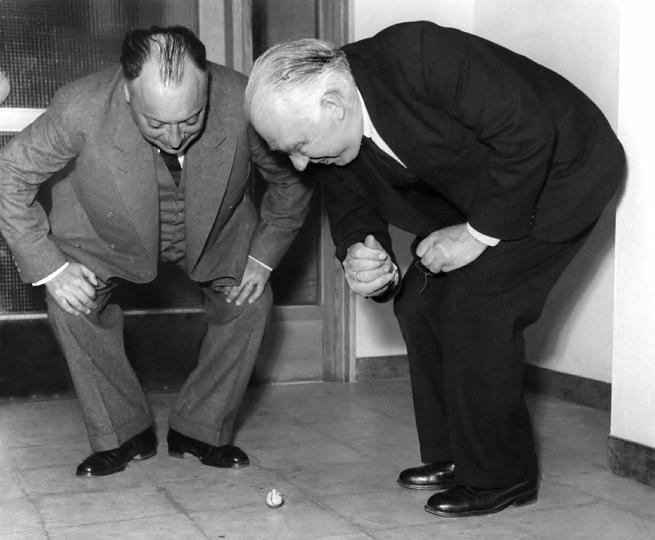
\includegraphics[scale=0.37]{Pauli_wolfgang_c4}
    \caption[,,Medytacja nad wirującym bąkiem``, \cite{PauliBohr}]{,,Medytacja nad wirującym bąkiem``, \cite{PauliBohr} \red Rysunki pozycjonujemy korzystając z~opcji \texttt{[tp]\protect\footnotemark}. Jeśli ilustracja jest zaczerpnięta z~jakiegoś źródła podajemy je, jeśli przygotowana na jego podstawie, piszemy: (na podstawie \cite{PauliBohr}). Nie stawiamy kropki na końcu podpisu}
    \label{fig:PauliBohr}
\end{figure}

O swojej inspiracji pisze także R. Feynman, również noblista, w zbiorze swoich wspomnień pod tytułem ,,\guillemotright{}Pan raczy żartować, panie Feynman!\guillemotleft{} Przypadki ciekawego człowieka'' \cite{feynman2007pan}, w którym przytacza anegdotę jak zainteresowanie wirującym talerzem wpłynęło na jego karierę zawodową i otrzymanie nagrody Nobla. W Polsce popularnonaukowym propagatorem tego zagadnienia jest Arkadiusz Jadczyk, profesor Uniwersytetu Wrocławskiego, prowadzący bloga \cite{Jadczyk}, którego duża część poświęcona jest opisowi, w~przystępny sposób, zachowania bąków.

\noindent
[\ldots]

{\red
  Wstęp jest też dobrym miejscem do przytoczenia rzeczy pobocznych, ciekawostek, elementów, które są drugoplanowe, aczkolwiek zdaniem autora warte przytoczenia. W~przypadku obiektów numerowanych, takich jak zamieszczony na stronie~\pageref{fig:PauliBohr} rysunek~\ref{fig:PauliBohr},\label{odsylacze} odwołania do nich wykonujemy wykorzystując mechanizm odsyłaczy\footnotetext{\red W~zrozumieniu sposobu kontrolowania rozmieszczenia obiektów pływających w~rodzaju rysunków może pomóc krótki opis znajdujący się na stronie \cite{latex_floats}.} \texttt{\textbackslash label\{\}}-\texttt{\textbackslash ref\{\}}\footnote{\red Tak też postępujemy w~przypadku innych ,,numerowanych'' obiektów, w~rodzaju tabel, rozdziałów, podrozdziałów, równań (choć w~przypadku tych ostatnich wygodniej jest używać polecenia \texttt{\textbackslash eqref\{\}}, które automatycznie dodaje wokół numeru wymagane nawiasy). Więcej na temat numerowania równań znajduje się w~stopce~$^\text{\ref{stopka_numery}}$ na stronie~\pageref{stopka_numery}. By odwołać się do strony, na której znajduje się etykieta stosujemy polecenie \texttt{\textbackslash pageref\{\}.}}. Przytaczany rysunek powinien zostać zdefiniowany w~źródle dokumentu (z wykorzystaniem otoczenia \texttt{figure}) zaraz po podaniu pierwszego odwołania do niego. Definicji rysunku nie należy oddzielać pustą linią od poprzedzającego ją/następującego po niej tekstu, jeśli nie znajdujemy się na końcu akapitu. Do każdego umieszczonego w~pracy rysunku musi być odwołanie w~tekście -- czytelnik zwraca swoją uwagę na rysunek dopiero wtedy, gdy napotka do niego odwołanie w~tekście. Te same zasady dotyczą tabel (otoczenie \texttt{table}\footnote{\red które służy do wstawiania obiektów pływających typu tabela i~które w~sumie nie musi zawierać tabel sensu stricte -- do przygotowania tabeli samej w~sobie służy otoczenie \texttt{tabular}}).}

Badanie zagadnienia ruchu obrotowego brył sztywnych jest istotne z punktu widzenia robotyki, ze względu na wykorzystywanie elementów wirujących w konstrukcjach robotycznych na przykład jako napędy. Przykładem robota mobilnego z napędem, który może zostać zamodelowany jako bąk jest między innymi Hogger \cite{ryba} oraz Hogger$^2$ \cite{goral}. Opis badań nad robotami napędzanymi w ten sposób można znaleźć w \cite{JonMu,JonMu2}.

{\red
  Warto we wstępie napisać, dlaczego zajęliśmy się tematem. I~warto zarówno w~nim, jak i~w~całej pracy unikać ,,eleganckiego'' stylu wypowiedzi, gdyż najczęściej wychodzi z~niego styl ,,pompatyczny'', oraz żargonu oraz niepotrzebnego słowotwórstwa. Jeśli przytaczamy kilka źródeł w~jednym miejscu podajemy je w~pojedynczym poleceniu \texttt{\textbackslash cite\{\}} rozdzielając przecinkiem.}

Niniejsza praca ma na celu wprowadzić czytelnika w podstawy problemu ruchu obrotowego oraz jego analizy. W~jej ramach przygotowano system symulacji pozwalający na śledzenie wybranych modelów bąków i wykorzystania go do przeprowadzenia badań komputerowych oraz wizualizacji ich zachowań. Układ pracy jest następujący. W~drugim rozdziale przytoczony został podstawowy aparat matematyczny, wraz z jego interpretacją, niezbędny do zrozumienia pracy. W rozdziale trzecim scharakteryzowano podstawowe przypadki bąków, dla których jesteśmy w~stanie uzyskać rozwiązanie całkowite bądź częściowe, zostały również przedstawione różnice pomiędzy nimi. Rozdział czwarty zawiera analityczną analizę bąków Lagrange'a oraz Eulera, która została poparta symulacjami przedstawionymi w~rozdziale piątym. Rozdział szósty podsumowuje całość.

{\red
  Wstęp należy zakończyć podając jakie są cele i~zakres pracy, oraz jej układ.}


%\vspace*{2em}
%\todo[inline]{ Dodać cytaty do bąków w rozdziale "Czym jest bąk?" -- na przykład z encyclopedia of mathematics .}\\
